\subsection{Catalan Numbers}

1, 1, 2, 5, 14, 42, 132, 429, 1430, 4862, 16796, 58786, 208012, 742900, 2674440, 9694845, 35357670, 129644790, 477638700, 1767263190, 6564120420, 24466267020, 91482563640, 343059613650, 1289904147324, 4861946401452, 18367353072152, 69533550916004, 263747951750360, 1002242216651368.\\

\[C_n = \frac{1}{n+1}\binom{2n}{n} = \frac{(2n)!}{(n+1)!n!} = \prod_{k=2}^{n} \frac{n+k}{k}, \quad n \geq 0\]\\


Applications:
\begin{itemize}

\item $C_n$ counts the number of expressions containing n pairs of parentheses which are correctly matched.
    \[((()))  \qquad  ()(())  \qquad  ()()()  \qquad  (())()  \qquad  \dots \]


\item Successive applications of a binary operator can be represented in terms of a full binary tree. (A rooted binary tree is full if every vertex has either two children or no children.) It follows that $C_n$ is the number of full binary trees with n + 1 leaves:\\
\begin{center}
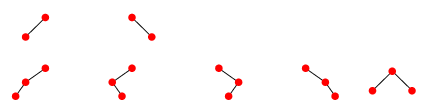
\includegraphics[width=0.85\linewidth]{img/catalan_tree.png}
\end{center}

\item $C_n$ is the number of different ways a convex polygon with n + 2 sides can be cut into triangles by connecting vertices with straight lines (a form of Polygon triangulation). The following hexagons illustrate the case n = 4:

\begin{center}

\includegraphics[width=\linewidth]{img/Catalan-Hexagons-example.png}
\end{center}

\end{itemize}
